% \section{Convolution Neural Networks Extended}
% A basic overview of the operations of Convolutional Neural Networks has been explained in the previous section. Some further points are explored below.

\subsection*{Receptive Field and Kernel}
In the previous section where an overview of CNN's was addressed, there was a discussion focused on filtering where features were searched for across the images.
This filtering resulted in windows sliding across the image, looking for common features.
This window is called the receptive field, and this is the section of the image that is being looked at.

As the image is convoluted and processed through the network, the changed image can be called the kernel.
The kernel of the CNN represents what features are extracted from the image throughout the network.

\subsection*{Activation Function}
The activation function used in a neural network calculates the output for a neuron.
The most commonly used activation function in CNN's is the ReLu activation function or the rectified linear unit \parencite{handsOnML}.
The SoftMax activation function is sometimes used for the output layer \parencite{handsOnML}.

\subsection*{Dropout}
Dropout is a type of regularisation technique used to prevent overfitting in a network \parencite{handsOnML}.
Overfitting in a network is when the network cannot generalise to new data after over learning the training data.
In dropout, each neuron is given a probability (normally set to 0.5) and this is the likelihood that the neuron will be used for that training step.
It has proven quite successful for increasing a networks accuracy \parencite{handsOnML}.

\subsection*{Full Connected Layer}
Once the layers of convolutional pooling have detected features in an image, a fully connected layer is added to the end of the CNN \parencite{fullyConnectedLayer}.
This layer uses the output of the previous layer to determine a prediction for the network.
The fully connected layer outputs a vector of n dimensions where n is the number of possible classes to predict.
A probability is calculated for each class to determine how likely it is that the class is present in the image.
This layer calculates the probabilities by looking for features in it's input that relate to the classes.
For example, if the image was of a banana the fully connected layer would look for features such as curved shape or yellow colour to calcukate a high probability.

\subsection*{Different Sizes of Convolutions}
Zero padding can be added to an output so that it is same size as the previous layer by adding zeros around the feature \parencite{handsOnML}..
Through training, it is " possible to connect a large input layer to a much smaller layer by spacing out the receptive fields" \parencite{handsOnML}.
The stride between two different receptive fields is the spacing between them \parencite{handsOnML}.

\subsection*{Fully Convolutional Networks}
A Fully Convolutional Network is one that does not have a fully connected layer
and in a fully connected layers place is another convolution layer.
This can be achieved by making the size of the receptive field equal to the size of the input \parencite{digits}.
They are proven to be very successful in object detection.

\subsection*{Inception-V3 Model Architecture}
The Inception V3 model network architecture was used for this experiment. The
Inception V3 architecture was created by building on the existing Inception
model aimed at efficient image classification \parencite{rethinkingInception}.
This research was carried out due to the popularity of convolutional neural networks.
The main aim of this study was to produce a model that would " scale up networks in ways that aim at utilizing the added computation as efficiently as possible by suitable factorized convolutions and aggressive regularization" \parencite{rethinkingInception}.
The team did not want to simply rely on larger models for better results.

The are 4 main design principles that the research team followed in the paper \parencite{rethinkingInception}:
\begin{itemize}
    \item{Avoid representational bottlenecks}
    \item{It is easier to process higher dimensional representations locally}
    \item{Without much loss in power, spatial aggregation can be carried out over lower dimensional embeddings}
    \item{The width and depth of the network should be balanced and when one is increased it can be beneficial to increase the other.}
\end{itemize}

\begin{figure}
     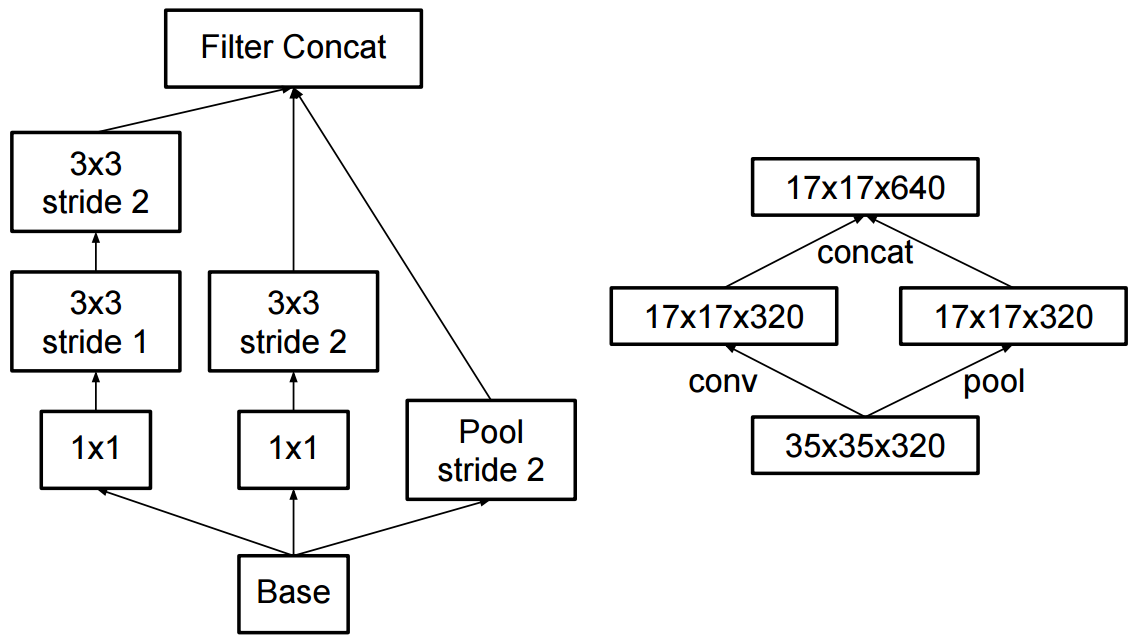
\includegraphics[scale=0.25]{inception}
     \caption{Inception module \parencite{rethinkingInception}}
     \label{fig:inception}
\end{figure}

The main idea behind the network is that different strands of the network are followed, and the best result is used as seen in Figure \ref{fig:inception}.

In order to combat the problem of low resolution input, three separate experiments were carried out based on the fact that "One simple way to ensure constant effort is to reduce the strides of the first two layer in the case of lower resolution input, or by simply removing the first pooling layer of the network" \parencite{rethinkingInception}.

These experiments are as follows, with the first (299 x 299 receptive field) resulting in the most accurate:
\begin{itemize}
    \item{"299 x 299 receptive field with stride 2 and maximum pooling after the first layer." \parencite{rethinkingInception}}
    \item{"151 x 151 receptive field with stride 1 and maximum pooling after the first layer." \parencite{rethinkingInception}}
    \item{"79 x 79 receptive field with stride 1 and without pooling after the first layer." \parencite{rethinkingInception}}
\end{itemize}

\begin{figure}
     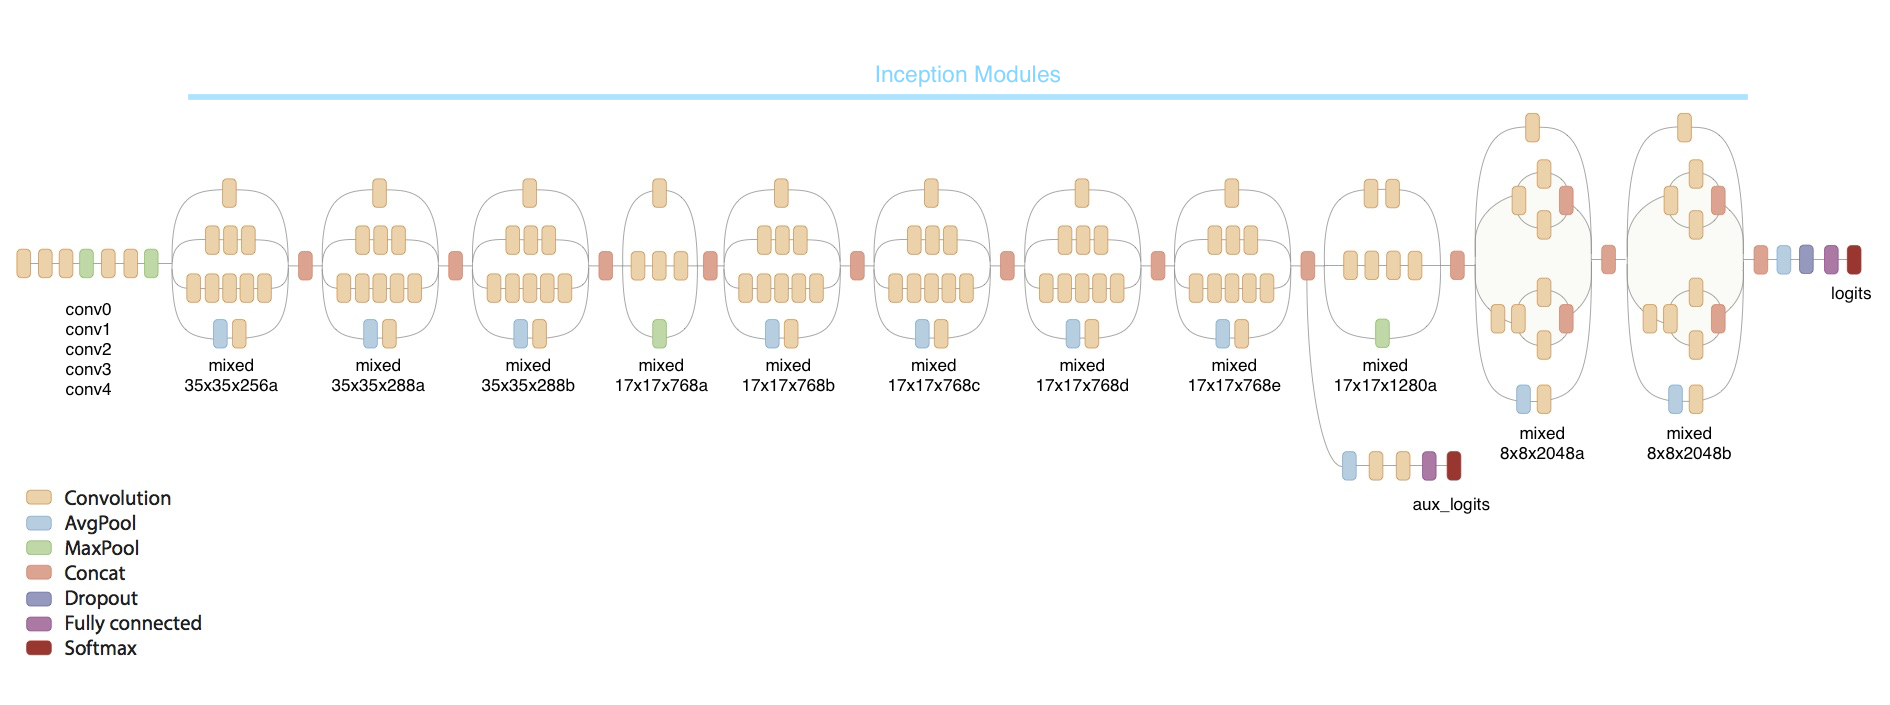
\includegraphics[scale=0.25]{inception_model}
     \caption{Inception V3 Architecture \parencite{rethinkingInception}}
     \label{fig:inception_model}
\end{figure}

The best results of the Inception-V3 model on the ILSVR 2012 dataset achieved 78.8\% Top-1 accuracy and 94.4\% Top 5 accuracy \parencite{rethinkingInception}.
This model also was the least computationally expensive of other published and successful models.
The full model can be viewed in Figure \ref{fig:inception_model}.

\subsection*{MobileNet Model Architecture}
The network architecture used for this experiment is MobileNet \parencite{mobilenet}.
A parameter can be set to retrain this model in the code, as mentioned in previous experiments, instead of inception V-3 \parencite{retrainInception}. 
This architecture is designed to be smaller and much more efficient so that
it can be used on smartphones which have less powerful resources available.

Mobilenet is designed for various use cases on mobile phones such as image classification, landmark recognition, object detection and face attributes.
It is based on " depthwise separable convolutions" whose purpose is the split a convolutional layer into a depthwise convolution and a pointwise convolution (1x1 convolution) \parencite{mobilenet}.
The purpose of the former is to apply " a single filter to each input channel" \parencite{mobilenet} while the latter combines these outputs.
This in turn reduces the computational time.
The first layer of the network is a standard convolutional layer and does not get split up.

Unfortunately there is a significant decrease in accuracy in using MobileNet as it is a much thinner model.

\subsection*{Libraries}
There are many libraries available that can be used for the creation of CNNs such as:
\begin{itemize}
    \item{TensorFlow}
    \item{Caffe}
    \item{Gluon}
    \item{MxNet}
\end{itemize}
In this project, TensorFlow will be used due to its reputation, supporting documentation, training resources and prevalence online.

\subsection*{History}
Convolutional Neural Networks are a bio-inspired approach to solving intensive tasks.
They have been applied to image recognition, along with natural language processing and voice recognition, with image recognition being explored since the 1980's \parencite{handsOnML}.
In 2012, CNNs increased in popularity due to increased computational power in the hardware, availability in datasets and breakthrough research carried out in the field \parencite{krizhevsky2012imagenet}.
CNNs have been recently applied to many complex tasks with exceptional results such as facial recognition, and many more.